%!TEX root = Slic3r-Manual.tex

Si le maillage 3D d\'ecrit dans le mod\`ele contient des trous, ou les bords ne sont pas align\'es (connu comme \'etant non-manifold), alors Slic3r peut avoir des probl\`emes de traitement . Slic3r va tenter de r\'esoudre les probl\`emes, s'il le peut, mais certains probl\`emes sont hors de sa port\'ee. Si l'application indique que le mod\`ele ne peut pas \^etre tranch\'e correctement alors il ya plusieurs options disponibles, et celles d\'ecrites ici sont tous libres au moment de l'\'ecriture.

%%% CONFIGURATION TUNING %%%
{%!TEX root = Slic3r-Manual.tex

\paragraph{Netfabb Studio} % (fold)
\label{par:netfabb_studio}
Netfabb produit une gamme d'applications de modélisation 3D, y compris une version de base gratuite\footnote{http://www.netfabb.com/basic.php}.  Cette version comprend un module de réparation de maillage qui peut aider à éliminer les différents problèmes rencontrés. Les instructions mise à jour peuvent être trouvés sur le wiki Netfabb\footnote{http://wiki.netfabb.com/Part\_Repair}, ce qui suit est un bref aperçu des étapes à suivre.

\begin{figure}[H]
\centering
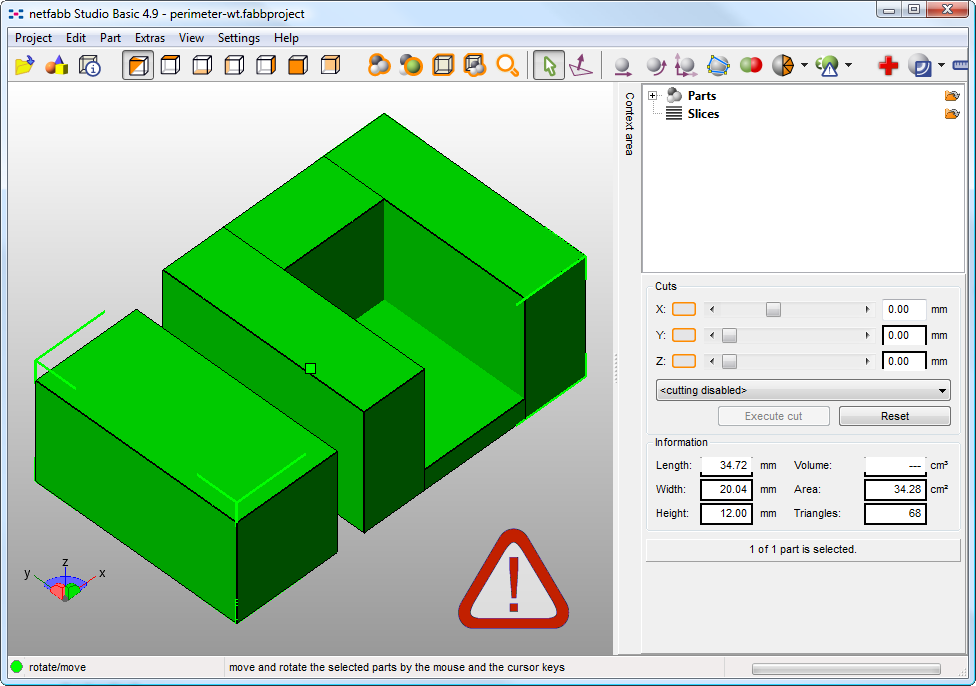
\includegraphics[keepaspectratio=true,width=0.75\textwidth]{working_with_models/netfabb_studio_part_repair.png}
\caption{Netfabb Studio: Réparation de modèle.}
\label{fig:netfabb_studio_part_repair}
\end{figure}

\begin{itemize}
	\item Lancer Netfabb studio, et charger le fichier STL qui a un problème, que ce soit par l'intermédiaire du menu \texttt{File} ou par glisser-déposer sur l'espace de travail. Si Netfabb détecte un problème, il affiche un signe d'alerte rouge dans le coin en bas à droite.
	\item Pour exécuter les scripts de réparation, sélectionnez la partie et puis cliquez sur la première icône d'aide dans la barre d'outils (la croix rouge), ou sélectionnez dans le menu contextuel \texttt{Extras->Repair Part}.  Cela va ouvrir l'onglet réparation de modèle et de montrer l'état du modèle.
	\item Les onglets \texttt{Actions} et \texttt{Repair scripts} offrent plusieurs scripts de réparation qui peuvent être appliquées manuellement, mais dans le but de cet aperçu sélectionez le script \texttt{Automatic repair} corrigera la plupart des problèmes.
	\item Le bouton de réparation automatique présente deux options: par défaut et simples. Choisir par défaut couvrira la plupart des cas. Selectionnez \texttt{execute} pour lancer le script.
	\item Une fois la pièce réparée les réparations doivent être appliquées en sélectionnant \texttt{Apply repair}, choisissant s'il faut passer outre la partie existante ou non.
	\item La pièce peut ensuite être exporté en sélectionnant \texttt{Export part->As STL} à partir du menu contextuel.
	\item Si Netfabb détecte encore que la partie exportée contient des erreurs, alors il offrira la possibilité d'appliquer d'autres réparations avant de l'exporter.
	\begin{figure}[H]
	\centering
	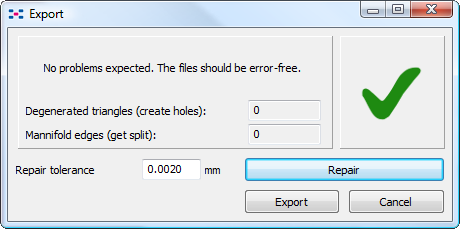
\includegraphics[keepaspectratio=true,width=0.75\textwidth]{working_with_models/netfabb_studio_export_part.png}
	\caption{Netfabb Studio: Export de pièce.}
	\label{fig:netfabb_studio_export_part}
	\end{figure}
\end{itemize}
% paragraph netfabb_studio (end)

\paragraph{Netfabb Cloud Service} % (fold)
\label{par:netfabb_cloud_service}
Netfabb accueille également un service web où un fichier STL peut être téléchargé pour être vérifié et réparé\footnote{http://cloud.netfabb.com/}.  

\begin{figure}[H]
\centering
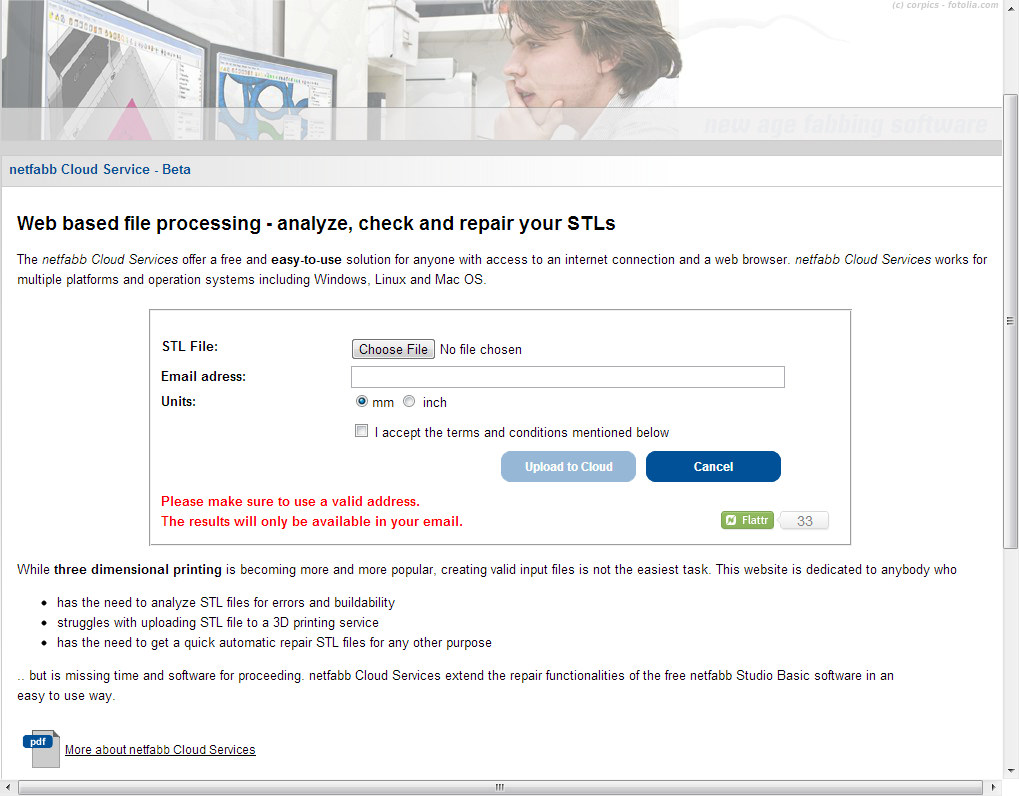
\includegraphics[keepaspectratio=true,width=0.75\textwidth]{working_with_models/netfabb_cloud_services.png}
\caption{Netfabb Cloud Services.}
\label{fig:netfabb_cloud_services}
\end{figure}

\begin{itemize}
	\item Accédez à http://cloud.netfabb.com
	\item Choisissez le fichier STL à télécharger en utilisant le bouton prévu.
	\item Une adresse e-mail doit être donnée pour vous informer quand la prestation est terminé.
	\item Choisissez entre les mesures métriques ou impériales qui doivent être utilisés.
	\item Lisez et acceptez les conditions de service, puis cliquez sur \texttt{Upload to Cloud}.
	\item Une fois que le service a analysé et réparé le fichier, un email est envoyé, fournissant le lien de téléchargement du fichier réparé.
\end{itemize}
}
%%% END CONFIGURATION TUNING %%%

\paragraph{FreeCAD} % (fold)
\label{par:freecad}
\index{FreeCAD}

Freecad\footnote{\url{http://sourceforge.net/projects/free-cad}} est un logiciel de CAO, complet et gratuit, qui est livr\'e avec un module de maillage, dans lequel on peut effectuer les r\'eparations d'erreur dans les mod\`eles. Les \'etapes suivantes d\'ecrivent comment un probl\`eme dans un fichier de mod\`ele peut \^etre analys\'e et r\'epar\'e.

\begin{figure}[H]
\centering
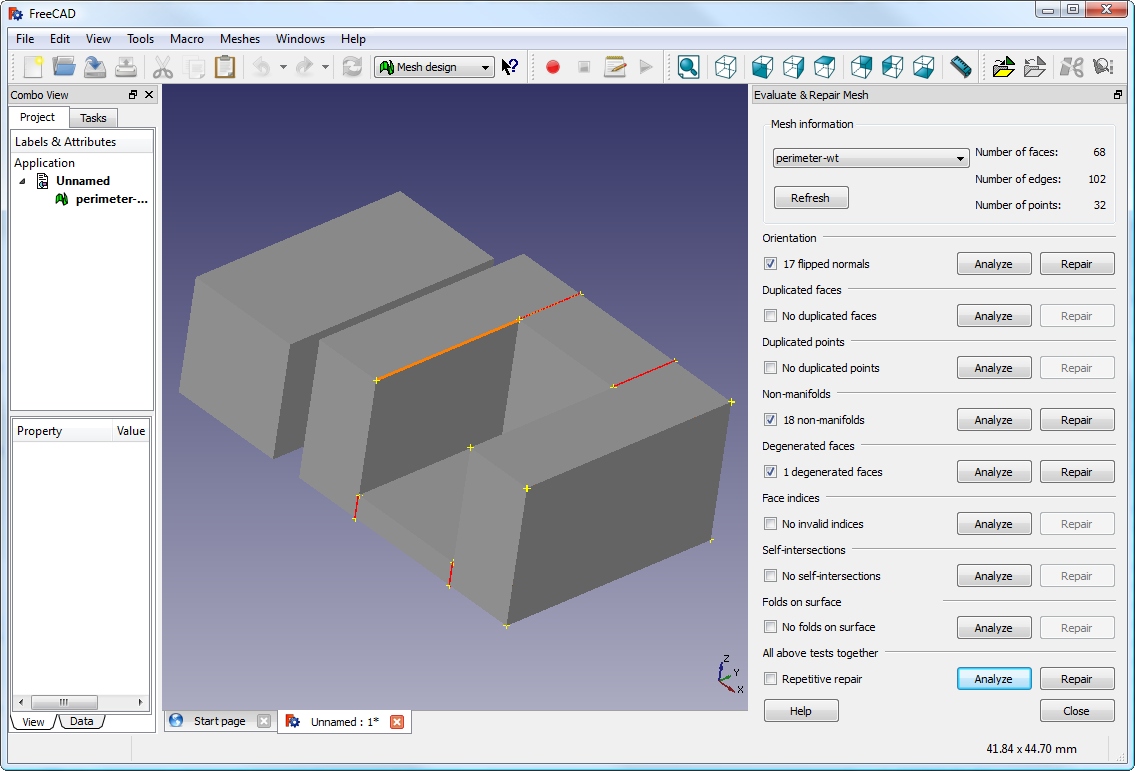
\includegraphics[keepaspectratio=true,width=0.75\textwidth]{working_with_models/freecad_part_repair.png}
\caption{R\'eparation avec FreeCAD.}
\label{fig:freecad_part_repair}
\end{figure}

\begin{itemize}
	\item Lancer FreeCAD et \`a partir la page d'accueil choisir \texttt{Working with Meshes}.
	\item Chargez le mod\`ele en le faisant glisser sur l'espace de travail ou par l'interm\'ediaire du menu \texttt{File}.  Un petit message dans le coin en bas \`a gauche indique si le mod\`ele semble avoir des probl\`emes.
	\item Dans le menu choisissez \texttt{Meshes->Analyze->Evaluate \& Repair mesh} pour faire appara\^itre la bo\^ite de dialogue des options de r\'eparation.
	\item Dans la bo\^ite de dialogue choisir la maille charg\'ee, puis effectuer chaque analyse soit en cliquant sur le bouton \texttt{Analyze} par type de probl\`eme, ou s\'electionnez \texttt{Repetitive Repair} en bas pour effectuer tous les contr\^oles. Si un probl\`eme  correspondant est d\'etect\'e le bouton \texttt{Repair} devient actif.
	\item Pour chaque r\'eparation souhait\'e frapp\'e le bouton \texttt{Repair}.
	\item Il est important d'examiner l'effet que le script de r\'eparation a apport\'ees au mod\`ele.  Il se peut que le script produise des dommages dans le fichier, plut\^ot que de le r\'eparer, par exemple en retirant triangles importants.
	\item Exporter le mod\`ele r\'epar\'e par le menu \texttt{Export} ou le menu contextuel.
\end{itemize}
% paragraph freecad (end)
